% -\textbf{}%\documentclass[a4paper,12pt]{upthesis}
\documentclass[a4paper,12pt]{upthesis}
\usepackage{graphicx}
\usepackage{amsmath}
\usepackage{amssymb}
\usepackage{chngcntr}

%\usepackage{natbib}
% แพคเกจสำหรับสร้าง hyperlink ด้วยคำสั่ง \href{<url>}{<Text to show>}
%\usepackage[linktocpage=true]{hyperref}       % Create hyperlink with command \href{<url>}{<Text to show>}.

% แพคเกจสำหรับเรียกใช้การหมุนภาพ หรือตาราง
\usepackage{rotating}       % Package for rotating either figure or table with command
                                      %\begin{sidewaysfigure} or \begin{sidewaystable} and also \end{} as well.
\usepackage{enumitem}		% For customize the symbols or enumeration                                      

% เป็นการกำหนดค่าเลขหน้าภาษาไทยในช่วงแรก
\usepackage{polyglossia}
\setdefaultlanguage{thai}
\setotherlanguages{thai}
% เป็นการกำหนดแพคเกจสำหรับจัดการเรื่องฟอนต์ รวมถึงการใช้ภาษาไทย
\usepackage{fontspec}
\usepackage{xunicode}
\usepackage{xltxtra}

\usepackage{indentfirst}
\usepackage{fancybox}
\usepackage{pst-grad}
\usepackage{pst-osci}
\usepackage{pst-coil}
\usepackage{tabularx}

% Set caption of Table & Figure align on the left most
% สำหรับกำหนดคำอธิบายของตารางและรูปให้อยู่ด้านซ้ายสุด
\usepackage[labelfont=bf, textfont=bf]{caption}
% labelfont = bf เป็นการกำหนดให้คำนำของตารางและรูปเป็นตัวหนา เช่น ตารางที่ 2 หรือ รูปที่ 3 จะเป็นตัวหนา เป็นต้น
% textfont = bf เป็นการกำหนดตัวอักษรคำอธิบายเป็นตัวหนา
% textfont = sl เป็นการกำหนดตัวอักษรคำอธิบายเป็นตัวเอียง
% singlelinecheck=off เป็นการกำหนดคำอธิบายที่มีบรรทัดเดียวให้เริ่มที่ด้านซ้ายสุด

% Set caption of Table & Figure align at start of Table or Figure LHS.
% กำหนดคำอธิบายตารางและภาพให้เริ่มต้นที่ด้านซ้ายมือสุดของตาราง หรือรูปภาพ
\usepackage{floatrow}
\floatsetup[table]{style=plaintop, footnoterule=none,footskip=.35\skip\footins}  
% Set caption of Table on top of table
% กำหนดคำอธิบายตารางให้อยู่ด้านบนของตาราง
% Use command \ttabbox {\caption {<caption text here>}} to set text equal a width of table.
% ใช้คำสั่ง \ttabbox {\caption {<caption text here>}} เพื่อกำหนดให้คำอธิบายมีขนาดความกว้างเท่ากับความกว้างของตาราง

% กำหนดการตัดคำ ขนาด และฟอนต์ที่จะใช้สำหรับภาษาไทย
\XeTeXlinebreaklocale "th_TH"
\XeTeXlinebreakskip = 0pt plus 1pt
\defaultfontfeatures{Scale=1.23}
\setmainfont[Mapping=tex-text]{TH Sarabun New}

%\setdefaultlanguage{thai}
%\newfontfamily{\thaifont}[Script=thai]{TH Niramit AS}

\usepackage{pstricks,pst-plot,pst-node}
\usepackage{pst-3dplot}
\usepackage{pstricks-add}

\usepackage{makeidx}         % allows index generation
\usepackage{graphicx}        % standard LaTeX graphics tool
                                             % when including figure files
\usepackage{multicol}         % used for the two-column index
\usepackage[bottom]{footmisc}% places footnotes at page bottom
\usepackage{tensor}             %for write tensor indices
\usepackage{color}                 % for assign a color to text with command
                                        %\textcolor{color}{text}
\usepackage{enumitem}		% For customize the symbols or enumeration                           

%Package for setup page (paper size)
% สำหรับการกำหนดขนาดของกระดาษ   *** แก้ไขได้ หากใช้กระดาษ และจัดขอบกระดาษต่างจากนี้ ***
\usepackage{geometry}
 \geometry{
 a4paper,		% Paper size ขนาดกระดาษ
 total={147.5mm,234.5mm},	% Total area of text on the page	ขนาดกว้างยาวของพื้นที่สำหรับข้อความในกระดาษ
 left=37.5mm,			% Left margin	1 inch = 25.4 mm ระยะขอบซ้าย
 %right=25mm,				% Right margin ระยะขอบขวา (ไม่กำหนดก็ได้ เพราะจะจัดอัตโนมัติ)
 top=37.5mm,			% Top margin	1.5 inch = 38.1 mm ระยะขอบบน
% bottom=25mm,		% Bottom margin ระยะขอบล่าง (ไม่กำหนดก็ได้ เพราะจะจัดอัตโนมัติ)
 }


% กำหนดรูปแบบสิ่งแวดล้อมของตัวอย่าง  *** ไม่ควรแก้ไข ***
\newcounter{Exampctr}\newsavebox{\Exampname}
\newenvironment{example}[1]
  {\stepcounter{Exampctr}%
   \sbox{\Exampname}{\textit{#1}}
   \begin{description}\item[ตัวอย่างที่ \arabic{Exampctr}][\usebox{\Exampname}]~}
   {\end{description}}

% กำหนดรูปแบบสิ่งแวดล้อมของนิยาม
\newcounter{Defctr}\newsavebox{\Defname}
\newenvironment{definition}[1]
  {\stepcounter{Defctr}%
   \sbox{\Defname}{\textit{#1}}
   \begin{description}\item[นิยาม \arabic{Defctr}][\usebox{\Defname}]~}
   {\end{description}}

% กำหนดรูปแบบสิ่งแวดล้อมของแบบฝึกหัด
\newcounter{Probctr}\newsavebox{\Probname}
\newenvironment{problem}[1]
  {\stepcounter{Probctr}
   \sbox{\Probname}{\textit{#1}}
   \begin{description}\item[แบบฝึกหัดที่ \arabic{Probctr}][\usebox{\Probname}]~}
   {\end{description}}

% กำหนดรูปแบบสิ่งแวดล้อมของทฤษฎีบท
\newcounter{Theoctr}\newsavebox{\Theoname}
\newenvironment{theorem}[1]
  {\stepcounter{Theoctr}
   \sbox{\Theoname}{\textit{#1}}
   \begin{description}\item[ทฤษฎีบทที่ \arabic{Probctr}][\usebox{\Theoname}]~}
   {\end{description}}

% การนิยามคำสั่งที่ใช้บ่อย และยาว ให้สั้นลง
\def\l{\left}
\def\r{\right}
%\def\be{\begin{equation}}
%\def\ee{\end{equation}}
%\def\bea{\begin{eqnarray}}
%\def\eea{\end{eqnarray}}
\def\f{\frac}
\def\no{\nonumber}
\def\i{\hat{i}}
\def\j{\hat{j}}
\def\k{\hat{k}}
\def\ro{\hat{\rho}}
\def\vp{\hat{\varphi}}
\def\x{\hat{x}}
\def\y{\hat{y}}
\def\z{\hat{z}}
\def\e#1{\hat{e}_{#1}}
\def\rh{\hat{r}}
\def\tt{\hat{\theta}}
\def\ph{\hat{\phi}}
\def\cross{\times}
\def\pd{\partial}
\def\pdx{\frac{\partial}{\partial x}}
\def\pdy{\frac{\partial}{\partial y}}
\def\pdz{\frac{\partial}{\partial z}}
\def\pdt{\frac{\partial}{\partial t}}
\def\ddx{\frac{d}{dx}}
\def\ddy{\frac{d}{dy}}
\def\ddz{\frac{d}{dz}}
\def\ddt{\frac{d}{dt}}
\def\pt#1#2{\frac{\partial{#1}}{\partial{#2}}}
\def\dd#1#2{\frac{d{#1}}{d{#2}}}
\def\det#1{\rm det({#1})}
\def\tr#1{\rm Tr({#1})}
\def\ul#1{\rm \underline{#1}}
\def\dul#1{\rm \underline{\underline{#1}}}
\def\mi#1#2{\rm M_{#1}(\underline{#2})}
\def\co#1#2{\rm C_{#1}(\underline{#2})}
\def\red#1{\textcolor{red}{#1}}
\def\blue#1{\textcolor{blue}{#1}}
\def\w9{{\rm WMAP9+BAO+}$H_0$}
\def\p15{$TT,TE,EE${\rm +lowP+Lensing+ext}}


% More references in gloss-thai of polyglossia package
% http://texdoc.net/texmf-dist/tex/latex/polyglossia/gloss-thai.ldf
% \thaiAlpha works well, the sequence is ก ข "ฃ" ค "ฅ" ฆ ง จ ...
% Normally, we need ก ข ค ง จ which is defined in \thaialph
% I'm not sure why it doesn't work. So, I just re-define it.
\def\thaialph#1{\expandafter\thalph\csname c@#1\endcsname}
\def\thalph#1{%
    \ifcase#1\or ก\or ข\or ค\or ง\or จ\or ฉ\or ช\or ซ\or
    ฌ\or ญ\or ฎ\or ฏ\or ฐ\or ฑ\or ฒ\or ณ\or ด\or ต\or ถ\or ท\or ธ\or น\or
    บ\or ป\or ผ\or ฝ\or พ\or ฟ\or ภ\or ม\or ย\or ร\or ฤ\or ล\or ฦ\or ว\or
    ศ\or ษ\or ส\or ห\or ฬ\or อ\else ฮ\else\xpg@ill@value{#1}{thalph}\fi}

\usepackage{subcaption}
%\renewcommand{\figurename}{รูปที่}
% กำหนดให้ subfigurename เป็น (ก), (ข), (ค), ...
\renewcommand{\thesubfigure}{\thaialph{subfigure}}	

%\renewcommand{\chaptername}{บทที่}
%\renewcommand{\figurename}{รูปที่}
%\renewcommand{\contentsname}{สารบัญ}
%\renewcommand{\indexname}{ดัชนี}

%%%%%%%%%%%%%%%
% Add prefix in front of Chapter number in Content
\usepackage{afterpage}
\DeclareRobustCommand*{\contheading}{%
  \afterpage{{\normalfont\large\bfseries\centering
 {\large\bf สารบัญ (ต่อ)}\\
 \hspace{10mm}{\normalsize\bf บทที่}\hfill {\normalsize\bf หน้า}\par\vspace{0.7cm}}}}
%%%%%%%%%%%%%%%
\DeclareRobustCommand*{\figcontheading}{%
  \afterpage{{\normalfont\large\bfseries\centering
 {\large\bf สารบัญภาพ (ต่อ)}\\ \vspace{0.5cm}
 \hspace{10mm}{\normalsize\bf ภาพ}\hfill {\normalsize\bf หน้า}\par\vspace{0.7cm}}}}
 %%%%%%%%%%%%%%%
\DeclareRobustCommand*{\tabcontheading}{%
  \afterpage{{\normalfont\large\bfseries\centering
 {\large\bf สารบัญตาราง (ต่อ)}\\ \vspace{0.5cm}
 \hspace{10mm}{\normalsize\bf ตาราง}\hfill {\normalsize\bf หน้า}\par\vspace{0.7cm}}}}
 %%%%%%%%%%%%%%%%%%%%%%%%%%%%%%

%%%%%%%%%%%%%%%%%%% Make List of Figure (Continued) page %%%%%%%%%%%%%%%%%%
\makeatletter



%%%%%%%%%%%%%%%%%%%%%%%%%%%%%%%%%%%%%%%

% สร้างดัชนีคำ (ถ้ามี) ก็ให้เอา % หน้า \makeindex ออก
%\makeindex             % used for the subject index
                       % please use the style svind.ist with
                       % your makeindex program

% สร้างเส้นหนาให้กับเส้นแนวนอน และเส้นแนวตั้งของตาราง
% ด้วยคำสั่ง \thline{1pt} หรือ \tvline{1pt}   %***ไม่ควรแก้ไข ***
% Make a Thick hline and vline in a Table
% by using \thline{1pt} or \tvline{1pt}
\usepackage{array,tabularx}
\makeatletter
\def\thline#1{%
    \noalign {\ifnum 0=`}\fi \hrule height #1
    \futurelet \reserved@a \@xhline
}
\def\tvline#1{@{\hskip\tabcolsep\vrule width #1\hskip\tabcolsep}}
\makeatother
% End of make thick hline and vline

% package{multirow} ใช้รวมแถวในตาราง
%package{multirow} is use to combine the rows in a table.
\usepackage{multirow}
% package{array} ใช้ขยายความสูงของแต่ละแถวในตาราง
%package{array} is use to expand the height of each row in a table.
\usepackage{array}
%This command is use to setting the stretch of the height of each row in a table.
% คำสั่งสำหรับตั้งค่าความสูงของแต่ละแถวในตาราง
%\renewcommand{\arraystretch}{2}
%\usepackage{fancyhdr}   % Customized the heading with command \lhead{}, \rhead{}, \chead{}, \lfoot{}, \rfoot{}, \cfoot{}
%\DeclareRobustCommand*{\contheading}{%
%  \afterpage{{\normalfont\large\bfseries\centering
%  สารบัญ (ต่อ)\par\bigskip}}}
% spacing after headings
%the titlesec package- it provides the command \titlespacing which has the format
%\titlespacing{command}{left spacing}{before spacing}{after spacing}[right]
%From the titlesec package
% spacing: how to read {12pt plus 4pt minus 2pt}
%           12pt is what we would like the spacing to be
%           plus 4pt means that TeX can stretch it by at most 4pt
%           minus 2pt means that TeX can shrink it by at most 2pt
%       This is one example of the concept of, 'glue', in TeX
%\titlespacing\section{0pt}{12pt plus 4pt minus 2pt}{0pt plus 2pt minus 2pt}

%%%%%%%%%%%%%%%%%%%%%%%%%%%%%%%%%%%%%%%%%%%%%%%%%%%%%%%%%%%
%%    ผู้เขียนเล่มการศึกษาอิสระ สามารถทำการแก้ไขได้ตั้งแต่ส่วนนี้เป็นต้นไป
%%%%%%%%%%%%%%%%%%%%%%%%%%%%%%%%%%%%%%%%%%%%%%%%%%%%%%%%%%%

% กำหนดหัวข้อภาษาไทย

% Just only Thai Title!!! This will be used at the title of Abstract
\title{  						% Title in Thai ชื่อเรื่องภาษาไทย
แอปพลิเคชันจัดตารางเวรพยาบาล
}
\titleen{						% Title in English ชื่อเรื่องภาษาอังกฤษ
Application for Nursing shift scheduling 
}

% คำนำหน้าผู้เขียน
\nameprefix{นาย}
\nameprefixen{Mr.}

% ชื่อ และนามสกุลของผู้เขียน
% \author{Name}{Surname}
\author{สิรวิชญ์}{คำชุ่ม}
\authoren{Sirawit}{Kamchoom}


% ชื่ออาจารย์ที่ปรึกษา
\advisor{อาจารย์ธรรมรัตน์ ธรรมา}                    % advisor
\advisoren{Dr.Phongsaphat Rangdee}

% ชื่ออาจารย์ที่ปรึกษาร่วม
\coadvisor{อาจารย์วรกฤต แสนโภชน์}
\coadvisoren{Dr.Chonticha Kritpetch}

%ชื่อปริญญา
\degree{วิทยาศาสตรบัณฑิต}                                   % degree
\degreeen{Bachelor of Science}
%ชื่อย่อปริญญา
\degreeAbb{วท.บ.}                                               % degree (abbreviation)
\degreeAbben{B.Sc.}

%หลักสูตร หรือสาขาวิชา
\major{วิทยาการคอมพิวเตอร์}                                      % major
\majoren{Computer Science}

% ภาควิชา หรือสาขาวิชา
\dept{ภาควิชาฟิสิกส์}                      % department

% เดือน และปี พ.ศ. ที่สำเร็จการศึกษา
\date{ตุลาคม 2565}                                               % date

% ปีการศึกษา
\academicyear{2565}                                             % academic year

% คำสำคัญ ภาษาไทย  และภาษาอังกฤษ
\keywordsth{                                                      % keywords in Thai คำสำคัญ ภาษาไทย ควรมีแค่ 3-4 คำ
            จัดตารางเวรพยาบาล, จัดตาราง, เวรพยาบาล , เว็บแอปพลิเคชัน, พยาบาล
         }
\keywords{						% Keywords in English คำสำคัญ ภาษาอังกฤษ ไม่ควรยาวมาก และควรมีแค่ 3-4 คำ
			Chaplygin Gas, Dark Energy, Accelerating Universe, Phantom Power-Law
		}

%%%%%%%%%%%%%%%%%%%%%%%%%%%%%%%%%%%%%%%%%%%%%%%%%%%%%%%%%%%%%%%%%%%%%%%%
%%-----------------------------------------------
%%               some Biography                %%
%%            ข้อมูลประวัติส่วนตัว					%%
%%-----------------------------------------------
% your birth date วันเดือนปีเกิด
\dateofbirth{20 มิถุนายน 2546}
% place of your birth  สถานที่เกิด
\placeofbirth{จังหวัดแม่ฮ่องสอน, ประเทศไทย}
% present address (province and country)	จังหวัดปัจจุบัน และประเทศ
\provinceTH{จังหวัดเชียงราย, ประเทศไทย}                  
% your current address	ที่อยู่ตามทะเบียนบ้าน หรือที่ติดต่อได้
\address{เลขที่ 182 หมู่ 6 ตำบลผางาม อำเภอเวียงชัย จังหวัดเชียงราย}
\zipcode{57210}		% รหัสไปรษณีย์
% Phone number  เบอร์โทรปัจจุบัน
\myphone{099-6633516}
% Email อีเมลที่ใช้อยู่
\myemail{sirawit.code@gmail.com}

% your working place สถานที่ทำงาน (ถ้ามี)
%\workplace{}
%\position{Lecturer at University of Phayao}
%\workplace{Department of Physics, Faculty of Science, University of Phayao, Phayao 56000, Thailand}

% Work Experiences ประสบการณ์การทำงาน (ถ้ามี)
%\WorkExpr{      
%\workexpr{2005 - 2009}{Lecturer at Department of Physics, Faculty of Science, University of Phayao, Phayao, Thailand}
%\workexpr{2000 - 2001}{Lecturer at Department of Physics, Faculty of Science, Naresuan University, Phitsanulok, Thailand}
%}

% Education Background การศึกษาที่ผ่านมา
\EduBG{         
\authorEduBG{มัธยมศึกษาตอนต้น}{โรงเรียนสามัคคีวิทยาคม อำเภอเมือง จังหวัดเชียงราย}{2560}
\authorEduBG{มัธยมศึกษาตอนปลาย}{โรงเรียนสามัคคีวิทยาคม อำเภอเมือง จังหวัดเชียงราย}{2563}
}

%Publication List  รายการผลงานตีพิมพ์ (ถ้ามี)
%\Publication{   
%\publication{1}{\textbf{Rachan Rangdee} (IF) and Burin Gumjudpai (IF and ThEP), ``Tachyonic (phantom) power-law cosmology'', Astrophysics and Space Science \textbf{349} (2014) 975-984.
%[arXiv:1210.5550 [astro-ph.CO]]}
%\publication{2}{Burin Gumjudpai (IF and ICTP) and \textbf{Phongsaphat Rangdee} (IF), ``Non-minimal derivative coupling gravity in cosmology'', General Relativity and Gravitation \textbf{47} (2015) 140.
%[arXiv:1511.00491 [gr-qc]]}
%}

% Oral and Poster Presentation List  รายการการนำเสนอทั้งแบบ Oral & Poster
%\Presentation{          
%\presentation{1}{\textbf{Rachan Rangdee} and Burin Gumjudpai (IF), ORAL ``Non-minimal Derivative Coupling with Power-Law'', RGJ-Ph.D. Congress XVI ``ASEAN: Emerging Research Oppotunities'', Pattaya, Chonburi, Thailand (2015).}
%\presentation{2}{\textbf{Rachan Rangdee} (IF), ORAL ``Aspects of non-minimal derivative coupling'', the $7^{\rm th}$ Aegean Summer School Beyond Einstein's Theory of Gravity, Parikia, Island of Paros, Greece, (2013).}
%\presentation{3}{\textbf{Rachan Rangdee} (IF), ORAL ``Tachyonic Phantom Power-Law Cosmology'', the Workshop on Heavy Ion and High Energy Physics 2012 (HIHEP2012), Naresuan University, Phitsanulok, Thailand (2012).}
%\presentation{4}{\textbf{Rachan Rangdee} (IF), ORAL ``Tachyonic Power-Law Cosmology'', the Siam Physics Congress 2012 (SPC2012): Past, Present and Future of Physics, Phranakhon Si Ayutthaya, Thailand (2012).}
%\presentation{5}{\textbf{Rachan Rangdee} (TPTP), POSTER ``TACHYONIC DARK ENERGY MODEL: DYNAMICS AND EVOLUTION'', the $11^{\rm th}$ Asian-Pacific Regional IAU Meeting (APRIM2011), Chiang Mai, Thailand (2011).}
%}

%%%%%%%%%%%%%%%%%%%%%%%%%%%%%%%%%%%%%%%%%%%%%%%%%%%%%%%%%%%%%%%%%%%%%%
%%%  เริ่มต้นเอกสาร
%%%%%%%%%%%%%%%%%%%%%%%%%%%%%%%%%%%%%%%%%%%%%%%%%%%%%%%%%%%%%%%%%%%%%%

\begin{document}

\pagenumbering{thaialph}
%\maketitle
%\newpage
%%%%%%%%%%%%%%%%%%%%%%%%%%%
%%%
%%% MAKE A COVER PAGE
%%% สร้างหน้าปก (หน้าแรก)
%%%%%%%%%%%%%%%%%%%%%%%%%%%%%

\thispagestyle{empty}
\begin{center} % กำหนดชื่อเรื่อง ภาษาไทย และภาษาอังกฤษ
\Large{\textbf{แอปพลิเคชันจัดตารางเวรพยาบาล\\
(Application for Nursing shift scheduling)\\}}
\vspace{7cm}
\textbf{นายสิรวิชญ์ คำชุ่ม\\} % ชื่อนามสกุลผู้เขียน
\vspace{7cm}
\textbf{ภาคนิพนธ์เสนอมหาวิทยาลัยพะเยา เพื่อเป็นส่วนหนึ่งของการศึกษา\\
หลักสูตรปริญญาตรี วิทยาศาสตร์บัณฑิต\\
สาขาวิชาวิทยาการคอมพิวเตอร์\\
ลิขสิทธิ์เป็นของมหาวิทยาลัยพะเยา}
\end{center}

%%%%%%%%%%%%%%%%%%%%%%%%%%%%%%%%%%%%%%%%%%%%%%%%%%%%%%%%%%%%%%%%%%%%%%%%

%%%%%%%%%%%%%%%%%%%%%%%%%%%
%%%
%%% MAKE AN APPROVE PAGE สร้างหน้าอนุมัติ
%%%
%%%%%%%%%%%%%%%%%%%%%%%%%%%%%

\newpage
\setcounter{page}{1}
\thispagestyle{empty}

% ใส่ชื่อเรื่องการศึกษาอิสระ
อาจารย์ที่ปรึกษาและประธานหลักสูตรวิทยาศาสตร์บัณฑิต สาขาวิชาวิทยาการคอมพิวเตอร์
คณะเทคโนโลยีสารสนเทศและการสื่อสาร มหาวิทยาลัยพะเยาได้พิจารณาภาคนิพนธ์ เรื่อง “แอปพลิเคชันจัดตารางเวรพยาบาล” เห็นสมควรรับ เป็นส่วนหนึ่งของการศึกษารายวิชา 225492 โครงงานวิทยาการคอมพิวเตอร์ ภาคการศึกษาต้น ปีการศึกษา 2567 มหาวิทยาลัยพะเยา
%Has been approved by the Graduate School as partial fulfillment of the requirements
%for the Doctor of Philosophy Degree in Theoretical Physics\\ of Naresuan University.\\
\vskip0.6cm
\normalsize
\begin{center}
%\textbf{คณะกรรมการสอบ}\vskip1cm
%\textbf{Oral Defense Committee}\vskip1cm
\vskip2.0cm

...........................................................................\\
(อาจารย์ธรรมรัตน์ ธรรมา)\\		% ใส่ชื่อประธานกรรมการสอบ
อาจารย์ที่ปรึกษา \\ 
\vskip2.0cm

...........................................................................\\
(ดร.กนกวรรธน์ เซี่ยงเจ็น)\\		% ใส่ชื่อประธานกรรมการสอบ
อาจารย์ที่ปรึกษา \\ 
\vskip2.0cm

...........................................................................\\
(อาจารย์วรกฤต แสนโภชน์)\\			% ใส่ชื่อกรรมการ คนที่เป็นอาจารย์ที่ปรึกษาหลัก
กรรมการ \\ 	
\vskip2.0cm

...........................................................................\\
(อาจารย์วรกฤต แสนโภชน์)\\			% ใส่ชื่อกรรมการ คนที่เป็นอาจารย์ที่ปรึกษาร่วม 
กรรมการ \\ 
\vskip2.0cm


%\textbf{ตรวจสอบแล้ว}\vskip1cm

...........................................................................\\
(อาจารย์ธนวัฒน์ แซ่เอียบ)\\
ประธานหลักสูตรวิทยาศาสตร์บัณฑิต สาขาวิทยาการคอมพิวเตอร์\\
คณะเทคโนโลยีสารสนเทศและการสื่อสาร มหาวิทยาลัยพะเยา \\
%\afterpage{\blankpage}
%\copyrightpage
\end{center}
\clearpage

%%%%%%%%%%%%%%%%%%%%%%%%%%%%%%%%%%%%%%%%%%%%%%%%%%%%%%%%%%%%%%%%%%%%%%%%

%%%%%%%%%%%%%%%%%%%%%%%%%%%
%%%
%%% MAKE AN ACKNOWLEDGEDMENT PAGE
%%% สร้างกิตติกรรมประกาศ จะขอบคุณใคร อะไร ก็ใส่ตรงนี้
%%%%%%%%%%%%%%%%%%%%%%%%%%%%%
\newpage
%\addtocontents{toc}{\protect\contentsline{chapter}{กิตติกรรมประกาศ}{\thepage}\protect}
\begin{acknowledgement}     % acknowledgement environment, this is optional
\baselineskip=8mm
\setcounter{page}{2}

ในการศึกษาวิจัยครั้งนี้ ข้าพเจ้าขอขอบพระคุณ ...

\vspace{0.5cm}
% or \input{acknowledgement.tex} % you need a separate acknowledgement.tex file to include it.
\begin{flushright}
\makeauthor
\end{flushright}

\end{acknowledgement}


\renewcommand{\arraystretch}{1.1}

%%%%%%%%%%%%%%%%%%%%%%%%%%%%%%%%%%%%%%%%%%%%%%%%%%%%%%%%%%%%%%%%%%%%%%%%

%%%%%%%%%%%%%%%%%%%%%%%%%%%
%%%
%%% MAKE AN ABSTRACT PAGE
%%% สร้างบทคัดย่อ ภาษาไทย และภาษาอังกฤษ
%%%%%%%%%%%%%%%%%%%%%%%%%%%%%
\newpage
%\addtocontents{toc}{\protect\contentsline{chapter}{บทคัดย่อ}{\thepage}\protect}
\begin{abstractth}	% เขียนบทคัดย่อภาษาไทย

บทคัดย่อภาษาไทย เขียนตรงนี้


\end{abstractth}

\newpage

%\maketitle
\renewcommand{\arraystretch}{1}

%%%%%%%%%%%%%%%%%%%%%%%%%%%%%%%%%%%%%%%%%%%%%%%%%%%%%%%%%%%%%%%%%%%%%%%%

%\newpage
% ถ้ามีคำนำ ก็สามารถเรียกใช้ตรงนี้ได้เลย
%

\begin{center}
\large{\textbf{คำนำ}}
\end{center}
\addcontentsline{toc}{chapter}{คำนำ}

เอกสารประกอบการสอน รายวิชา 244211 กลศาสตร์ 1 (Mechanics I) จำนวนหน่วยกิต 3(3-0-6) หน่วยกิต เป็นรายวิชาที่เปิดสอนสำหรับนิสิต หลักสูตรวิทยาศาสตรบัณฑิต สาขาวิชาฟิสิกส์ และนิสิตหลักสูตรการศึกษาบัณฑิต สาขาวิชาการศึกษา และหลักสูตรวิทยาศาสตรบัณฑิต สาขาวิชาฟิสิกส์ ชั้นปี 2 มหาวิทยาลัยพะเยา โดยมี ข้าพเจ้า นายพงศพัศ แรงดี เป็นผู้สอน และผู้จัดการรายวิชา

ในเอกสารประกอบการสอนนี้ เป็นเนื้อหาที่ใช้ในการเรียนการสอนของวิชากลศาสตร์ 1 ซึ่งเนื้อหาต่างๆนั้น จะแยกเป็นบทๆ พร้อมทั้งมีแบบฝึกหัดให้ลองทำในท้ายหัวข้อย่อยแต่ละหัวข้อ โดยหัวข้อหลักๆ ประกอบไปด้วย เวกเตอร์ และการดำเนินการเวกเตอร์ขั้นสูง กฎการเคลื่อนที่ของนิวตัน กลศาสตร์นิวตันของอนุภาคเดี่ยวใน 1 มิติ 2 มิติ และ 3 มิติ การสั่น แรงศูนย์กลาง การเคลื่อนที่ในกรอบอ้างอิงไม่เฉื่อย การเคลื่อนที่ของระบบอนุภาค การเคลื่อนที่ของวัตถุแข็งเกร็ง กลศาสตร์ของไหล และจบเนื้อหาในเรื่อง กลศาสตร์แบบลากรองจ์และกลศาสตร์แบบแฮมิลตันเบื้องต้น และเนื้อหาทั้งหมดนี้ เป็นเนื้อหาที่ใช้ในการเรียนการสอนสำหรับ 1 ภาคการศึกษา

ผู้เขียนมีความคาดหวังว่า นิสิตที่อ่านเอกสารประกอบการสอนชุดนี้จะได้รับประโยชน์แก่ตนเอง โดยทำให้การเรียนวิชากลศาสตร์ 1 มีความเข้าใจมากยิ่งขึ้น และช่วยให้ทำคะแนนสอบได้ดีขึ้น อีกทั้งจะเป็นพื้นฐานสำหรับการเรียนรู้ในรายวิชาอื่นๆในระดับที่สูงขึ้นไปได้

หากท่านใดที่มีความสนใจจะศึกษาเพิ่มเติม นอกเหนือจากเนื้อหาในเอกสารประกอบการสอนเล่มนี้แล้ว ท่านสามารถค้นคว้าตามเอกสารในบรรณานุกรมได้ และหากมีข้อผิดพลาดประการใดผู้เขียนขอน้อมรับไว้แต่ผู้เดียว โดยหวังเป็นอย่างยิ่งว่าในฉบับพิมพ์ครั้งต่อไปจะพยายามลดข้อผิดพลาดให้เหลือน้อยที่สุด

%% Please "sign" your preface
\vspace{1cm}
\begin{flushleft}\noindent
มกราคม 2560 \hfill  พงศพัศ แรงดี
\end{flushleft}










   

%%%%%%%%%%%%%%%%%%%%%%%%%%%%%%%%%%%%%%%%%%%%%%%%%%%%%%%%%%%%%%%%%%%%%%%%
\newpage
% สร้างสารบัญ
\tableofcontents
% เพิ่มสารบัญเรื่อง ในสารบัญ
\clearpage

%%%%%%%%%%%%%%%%%%%%%%%%%%%%%%%%%%%%%%%%%%%%%%%%%%%%%%%%%%%%%%%%%%%%%%%%

% List of Tables
% สร้างสารบัญตาราง
\listoftables
% เพิ่มสารบัญตารางในสารบัญ
\clearpage

%%%%%%%%%%%%%%%%%%%%%%%%%%%%%%%%%%%%%%%%%%%%%%%%%%%%%%%%%%%%%%%%%%%%%%%%

%List of Figures
% สร้างสารบัญภาพ
\listoffigures
% เพิ่มสารบัญภาพในสารบัญ
\clearpage

%%%%%%%%%%%%%%%%%%%%%%%%%%%%%%%%%%%%%%%%%%%%%%%%%%%%%%%%%%%%%%%%%%%%%%%%

% กำหนดเลขหน้าเป็นเลขอารบิก
\pagenumbering{arabic}
\pagestyle{headings}
\setcounter{page}{1}

\newpage

%%%%%%%%%%%%%%%%%%%%%%%%%%%%%
%%%
%%% ADD CHAPTER TO THE MAIN FILE เพิ่มเนื้อหาของแต่ละบท
%%%
%%%%%%%%%%%%%%%%%%%%%%%%%%%%%

\setcounter{secnumdepth}{4}
\numberwithin{equation}{chapter}
\numberwithin{equation}{section}
\baselineskip=8mm
\chapter{บทนำ}

% \renewcommand{\thesubsection}{\thechapter.\arabic{subsection}}
\renewcommand{\thesubsection}{\arabic{subsection}.}
\renewcommand{\theequation}{\thesection\arabic{equation}}
\renewcommand{\thesubsubsection}{\thesubsection\arabic{subsubsection}}
\renewcommand{\thesection}{}
\renewcommand{\paragraph}{}
\section{ที่มาและความสำคัญของปัญหา}

เนื่องจากสถานการณ์การแพร่ระบาดของโรคติดเชื้อไวรัสโคโรนา 2019 (Covid -19) จากเมืองอู่ฮั่น(Wuhan) มณฑลหูเป่ย(Hubei) ประเทศสาธารณรัฐประชาชนจีน ทำให้มีการแพร่ระบาดขยายเป็นวงกว้างอย่างรวดเร็วไปยังประเทศต่างๆทั่วโลกรวมถึงประเทศไทยด้วย ทำให้ส่งผลกระทบต่อสาธารณสุข เศรษฐกิจ สังคม \cite{wuhan:hupei}
พยาบาลเป็นหนึ่งในทีมบุคลากรทางการแพทย์ที่มีบทบาทเป็นด่านหน้าในการควบคุมและป้องกันการแพร่ระบาดของโรค เป็นผู้ปฏิบัติงานโดยตรงกับผู้ป่วยต้องเข้าไปสัมผัสใกล้ชิดกับผู้ป่วย พยาบาลต้องตระหนักและดูแลป้องกันตนเองไม่ให้ติดเชื้อต้องมาตรฐานอย่างเคร่งครัด \cite{nurse:covid}
ทำให้พยาบาลเกิดความเหนื่อย ความเครียดจากภาระงานที่เพิ่มมากขึ้น ในการปฏิบัติงานพยาบาลต้องดูแลผู้ป่วยใน Home Isolation ที่ต้องรับคำปรึกษาตลอดเวลาและขึ้นเวร Community Isolation โรงพยาบาลสนามโดยไม่ได้หยุดพัก \cite{nurse:Isolation}
เมื่อเปรียบเทียบจำนวนพยาบาลกับสัดส่วนประชากรโดยมากถึง 1 : 353 \cite{people:nurse} ความเหนื่อยล้าจากการทํางานของพยาบาลส่งผลกระทบต่อ ความปลอดภัยของผู้ป่วยที่ลดลง การดูแลเอาใจใส่ผู้ป่วยที่อาจไม่ดีเท่าที่ควร พยาบาลต้องทํางานต่อเนื่องกันยาวนานถึง 12 ชั่วโมงอาจทําให้เกิดอัตราความผิดพลาดจากการทํางานเพิ่มขึ้น \cite{ngeaun:nurse}
โดยปกติแนวทางในการจัดตารางเวรของพยาบาลจะยึด แนวทางการบริหารการจัดตารางเวรหรือผลัด การเบิกเงินค่าตอบแทนนอกเวลา และค่าเวรหรือผลัด ของพยาบาลวิชาชีพ พยาบาลเทคนิค ผู้ช่วยพยาบาล กระทรวงสาธารณสุข เป็นหลักแต่สามารถปรับแต่งการจัดจัดตารางเวรให้เหมาะสมได้ \cite{tarang:nurse}
โดยการจัดตารางเวรหัวหน้าพยาบาลจะเป็นผู้จัดทำ การจัดตารางเวรแบบเดิมจะใช้การจดบันทึกในการดาษและเนื่องจากปัจจุบันเทคโนโลยีได้เข้ามามีบทบาทอย่างมากจึงเกิดการประยุกต์ใช้เทคโนโลยีเพื่อจัดตารางเวรของพยาบาล อาทิเช่นแอปพลิเคชัน “Microsoft Excel” ที่มาช่วยในการจัดตารางให้ดูง่ายสามารถคำนวณวันเวลาได้ลดความยุ่งยากในการจัดเก็บเอกสาร \cite{excel:headnurse}

จากการจัดตารางเวรข้างต้นของหัวหน้าพยาบาลแสดงให้เห็นว่าการจัดตารางเวรแบบเดิมหรือการจัดตารางเวรโดยการใช้แอปพลิเคชัน “Microsoft Excel” ก็ยังคงเกิดปัญหาในหลายๆเรื่อง เช่น การจัดตารางเวรจัดไม่เท่ากัน โดยอาจเกิดการเองเอียง ความเหลื่อมล้ำ โดยหัวหน้าพยาบาลไม่ได้มีข้อมูลในการชี้แจงที่ชัดเจน การจัดตารางเวรอาจไม่ได้ตรงตามความต้องการของพยาบาล ทำให้พยาบาลอาจมีการแลกเวรจำนวนมากๆ ซึ่งส่งผลให้การจัดตารางเวรนั้นเปลี่ยนไม่ตรงตามวัตถุประสงค์ที่หัวหน้าพยาบาลต้องการตั้งแต่ตั้น ข้อมูลตารางเวรหากมีการเปลี่ยนแปลงโดยการแลกเวรจะต้องทำการอัปเดตซึ่งเป็นไปได้ยาก 

จากปัญหาข้างต้นเพื่อแก้ไขปัญหาดังกล่าว ผู้จัดทำมุ่งเน้นการพัฒนาระบบผ่านเว็บแอปพลิเคชันเพื่อให้พยาบาลสามารถเข้าถึงและจัดการตารางเวรได้อย่างง่ายดายผ่านอินเทอร์เน็ต ระบบนี้จะช่วยลดความยุ่งยากในการจัดตารางเวร ตอบสนองความต้องการของพยาบาลในการจัดตารางเวร อำนวยความสะดวกในการขอลาและการแลกเวร โดยสามารถอัปเดตข้อมูลตารางเวรได้ง่ายขึ้น โดยหัวหน้าพยาบาลจะมีข้อมูลเก่าในระบบที่สามารถนำมาวิเคราะห์เพื่อจัดตารางเวรหรือตอบคำถามให้พยาบาลได้ ซึ่งทำให้ลดการถกเถียงในการจัดตารางเวร และมีภาพรวมให้ผู้อำนวยการโรงพยาบาลได้ทราบก่อนที่จะอนุมัติตารางเวรได้จึงทำให้โรงพยาบาลมีระบบระเบียบ มีประสิทธิภาพมากยิ่งขึ้น

\section{{วัตถุประสงค์}}

\hspace{0cm}\subsection{เพื่อสร้างแอปพลิเคชันอำนวยความสะดวกให้กับหัวหน้าพยาบาลและให้พยาบาล}

\hspace{0cm}\subsection{เพื่อเป็นการศึกษาและพัฒนาเว็บแอปพลิเคชัน}

\section{แนวคิดและหลักการ}

แอปพลิเคชันจัดตารางเวรพยาบาลถูกออกแบบมาเพื่อศึกษาและหาวิธีแก้ปัญหาเกี่ยวกับการจัดการตารางเวรของพยาบาล เช่น การจัดตารางเวร การแลกเวร การลา และปัญหาอื่นๆที่เกี่ยวข้อง แอปพลิเคชันนี้ถูกออกแบบมาเป็นเว็บแอปพลิเคชันเพื่อความสะดวกในการใช้งาน ผู้ใช้สามารถเข้าถึงแอปพลิเคชันได้ง่ายผ่านอินเทอร์เน็ตโดยไม่ต้องติดตั้งโปรแกรมใดๆเพิ่มเติม ในการออกแบบระบบได้นำหลักการวิเคราะห์และออกแบบระบบมาใช้โดยใช้ทฤษฎีวงจรชีวิตการพัฒนาซอฟต์แวร์ (Software Development Lifecycle : SDLC)
หน้าตาส่วนต่อประสานกับผู้ใช้ (UI) ได้รับการออกแบบโดยคำนึงถึงความสะดวกในการใช้งาน ใช้งานง่าย เข้าใจง่าย สวยงาม และสอดคล้องกับหลักการออกแบบ UI ทั่วไป โครงสร้างของระบบถูกออกแบบโดยใช้แผนภาพยูเอ็มแอล (Unified Modeling Language : UML) ซึ่งเป็นเครื่องมือที่ใช้ในการวิเคราะห์ ออกแบบ และสร้างแบบจำลองระบบ ช่วยให้เข้าใจโครงสร้างของระบบได้ง่าย และสามารถนำไปพัฒนาต่อได้สะดวก จากการออกแบบแอปพลิเคชันจัดตารางเวรพยาบาล คาดว่าจะช่วยแก้ปัญหาเกี่ยวกับการจัดการตารางเวรของพยาบาล เพิ่มประสิทธิภาพการทำงาน และช่วยให้พยาบาลสามารถจัดการตารางเวรของตัวเองได้สะดวกยิ่งขึ้น
\clearpage

\section{ขอบเขตการศึกษา}
\setcounter{secnumdepth}{4}

ผู้จัดทำแอปพลิเคชันจัดตารางเวรพยาบาลได้ทำการเก็บข้อมูลและได้ทำการออกแบบฟังก์ชันตามระดับของผู้ใช้งานโดยมีขอบเขตการทำงานโดยแบ่งผู้ใช้ออกเป็น 5 ประเภทดังนี้


\hspace{0cm}\textbf{\subsection{\textbf{ผู้ดูแลระบบแอปพลิเคชัน}}}

\hspace{1cm}\subsubsection{จัดการข้อมูลการเข้าสู่ระบบ}

\hspace{2.5cm}\paragraph{1.1.1 สามารถเข้าสู่ระบบ}

\hspace{2.5cm}\paragraph{1.1.2 สามารถแก้ไข Username และ Password}

\hspace{2.5cm}\paragraph{1.1.3 สามารถเพิ่ม ลบ ผู้ใช้งานในระบบ}

\hspace{2.5cm}\paragraph{1.1.4 สามารถออกจากระบบ}

\hspace{1cm}\subsubsection{จัดการโรงพยาบาล}

\hspace{2.5cm}\paragraph{1.2.1 สามารถเพิ่ม ลบ แก้ไข ข้อมูลเทียบเท่าผู้ดูแลระบบของโรงพยาบาล}

\hspace{1cm}\subsubsection{ดูข้อมูลสถิติการใช้งาน}

\hspace{2.5cm}\hangindent=4.9cm\hangafter=1\paragraph{1.3.1 สามารถดูข้อมูลการใช้งานของแต่ละโรงพยาบาล เช่น จำนวนการแลกเวรเฉลี่ยของพยาบาล จำนวนพยาบาลต่อวอร์ดโดยเฉลี่ย เป็นต้น}


\hspace{1cm}\subsubsection{จัดการสิทธิการใช้งาน}

\hspace{2.5cm}\paragraph{1.4.1 กำหนดสิทธิการใช้งานของแต่ละผู้ใช้}




\hspace{0cm}\textbf{\subsection{\textbf{ผู้ดูแลระบบโรงพยาบาล}}}

\hspace{1cm}\subsubsection{จัดการข้อมูลการเข้าสู่ระบบ}

\hspace{2.5cm}\paragraph{2.1.1 สามารถเข้าสู่ระบบ}

\hspace{2.5cm}\paragraph{2.1.2 สามารถแก้ไข Username และ Password}

\hspace{2.5cm}\paragraph{2.1.3 สามารถเพิ่ม ลบ ผู้ใช้งานในระบบ}

\hspace{2.5cm}\paragraph{2.1.4 สามารถออกจากระบบ}

\hspace{1cm}\subsubsection{จัดการข้อมูลโรงพยาบาล}

\hspace{2.5cm}\paragraph{2.2.1 สามารถเพิ่ม ลบ แก้ไขข้อมูลของโรงพยาบาล}

\hspace{1cm}\subsubsection{จัดการข้อมูลวอร์ด}

\hspace{2.5cm}\paragraph{2.3.1 สามารถเพิ่ม ลบ แก้ไขข้อมูลวอร์ดของโรงพยาบาล}

\hspace{1cm}\subsubsection{ตั้งค่าระดับพยาบาล}

\hspace{2.5cm}\paragraph{2.4.1 สามารถตั้งค่าระดับพยาบาลของโรงพยาบาล}

\hspace{1cm}\subsubsection{ดูสถิติการทำงานของพยาบาล}

\hspace{2.5cm}\paragraph{2.5.1 สามารถดูข้อมูลสถิติการทำงานโดยภาพรวมของพยาบาล}





\hspace{0cm}\textbf{\subsection{\textbf{ผู้อำนวยการโรงพยาบาล}}}

\hspace{1cm}\subsubsection{จัดการข้อมูลการเข้าสู่ระบบ}

\hspace{2.5cm}\paragraph{3.1.1 สามารถเข้าสู่ระบบ}

\hspace{2.5cm}\paragraph{3.1.2 สามารถแก้ไข Username และ Password}

\hspace{2.5cm}\paragraph{3.1.3 สามารถออกจากระบบ}

\hspace{1cm}\subsubsection{การอนุมัติ}

\hspace{2.5cm}\paragraph{3.2.1 สามารถอนุมัติตารางเวรของพยาบาล}

\hspace{2.5cm}\paragraph{3.2.2 สามารถอนุมัติการลาของพยาบาล}

\hspace{1cm}\subsubsection{ดูสถิติการทำงานของพยาบาล}

\hspace{2.5cm}\paragraph{3.3.1 สามารถดูข้อมูลสถิติการทำงานของพยาบาล}







\hspace{0cm}\textbf{\subsection{\textbf{หัวหน้าพยาบาล}}}

\hspace{1cm}\subsubsection{จัดการข้อมูลการเข้าสู่ระบบ}

\hspace{2.5cm}\paragraph{4.1.1 สามารถเข้าสู่ระบบ}

\hspace{2.5cm}\paragraph{4.1.2 สามารถแก้ไข Username และ Password}

\hspace{2.5cm}\paragraph{4.1.3 สามารถออกจากระบบ}

\clearpage

\hspace{1cm}\subsubsection{จัดตารางเวร}

\hspace{2.5cm}\paragraph{4.2.1 สามารถจัดตารางเวรของพยาบาล}

\hspace{2.5cm}\paragraph{4.2.2 สามารถแก้ไขตารางเวรของพยาบาล}

\hspace{2.5cm}\paragraph{4.2.3 สามารถนำตารางออกเป็นไฟล์ PDF}

\hspace{1cm}\subsubsection{การอนุมัติ}

\hspace{2.5cm}\paragraph{4.3.1 สามารถอนุมัติการแลกเวรของพยาบาล}

\hspace{2.5cm}\paragraph{4.3.2 สามารถอนุมัติการลาของพยาบาล}

\hspace{1cm}\subsubsection{ตารางเวร}

\hspace{2.5cm}\paragraph{4.4.1 สามารถดูตารางเวรของตัวเองได้}

\hspace{1cm}\subsubsection{แลกเวร}

\hspace{2.5cm}\paragraph{4.5.1 สามารถแลกเวรกับพยาบาลคนอื่น}

\hspace{2.5cm}\paragraph{4.5.2 สามารถดูประวัติการแลกเวร}

\hspace{2.5cm}\paragraph{4.5.3 สามารถดูความคืบหน้าของการแลกเวรได้}

\hspace{2.5cm}\paragraph{4.5.4 สามารถยกเลิกการแลกเวร}


\hspace{1cm}\subsubsection{การลา}

\hspace{2.5cm}\paragraph{4.6.1 สามารถขอลาได้}

\hspace{2.5cm}\paragraph{4.6.2 สามารถดูประวัติการลาของตัวเองได้}

\hspace{2.5cm}\paragraph{4.6.3 สามารถดูความคืบหน้าของการลาได้}

\hspace{2.5cm}\paragraph{4.6.4 สามารถยกเลิกการลาได้}



\hspace{0cm}\textbf{\subsection{\textbf{พยาบาล}}}

\hspace{1cm}\subsubsection{จัดการข้อมูลการเข้าสู่ระบบ}

\hspace{2.5cm}\paragraph{5.1.1 สามารถเข้าสู่ระบบ}

\hspace{2.5cm}\paragraph{5.1.2 สามารถแก้ไข Username และ Password}

\hspace{2.5cm}\paragraph{5.1.3 สามารถออกจากระบบ}

\hspace{1cm}\subsubsection{ขอเวร}

\hspace{2.5cm}\paragraph{5.1.1 สามารถขอเวรได้}

\hspace{2.5cm}\paragraph{5.1.2 สามารถดูการขอเวรของพยาบาลคนอื่น}

\hspace{1cm}\subsubsection{ตารางเวร}

\hspace{2.5cm}\paragraph{5.2.1 สามารถดูตารางเวรของตัวเองได้}

\hspace{1cm}\subsubsection{แลกเวร}

\hspace{2.5cm}\paragraph{5.3.1 สามารถแลกเวรกับพยาบาลคนอื่น}

\hspace{2.5cm}\paragraph{5.3.2 สามารถดูประวัติการแลกเวร}

\hspace{2.5cm}\paragraph{5.3.3 สามารถดูความคืบหน้าของการแลกเวรได้}

\hspace{2.5cm}\paragraph{5.3.4 สามารถยกเลิกการแลกเวร}

\hspace{1cm}\subsubsection{การลา}

\hspace{2.5cm}\paragraph{5.4.1 สามารถขอลาได้}

\hspace{2.5cm}\paragraph{5.4.2 สามารถดูประวัติการลาของตัวเองได้}

\hspace{2.5cm}\paragraph{5.4.3 สามารถดูความคืบหน้าของการลาได้}

\hspace{2.5cm}\paragraph{5.4.4 สามารถยกเลิกการลาได้}

\vspace{0cm}

\begin{table}[h]
    \captionsetup{justification=raggedright,singlelinecheck=false}
    \centering
    \fontsize{8}{10}\selectfont	
    \resizebox{\textwidth}{!}{%
        \begin{tabular}{l c c c c c}
            \toprule
            \multicolumn{1}{c}{\multirow{2}{*}{ขอบเขตการทำงาน}} & \multicolumn{5}{c}{ระดับของผู้ใช้ในระบบ} \\ \cline{2-6} 
            \multicolumn{1}{c}{} & ผู้ดูแลระบบแอปพลิเคชัน & ผู้ดูแลระบบโรงพยาบาล & ผู้อํานวยการโรงพยาบาล & หัวหน้าพยาบาล & พยาบาล \\ \hline
            จัดการข้อมูลการเข้าสู่ระบบ & \checkmark & \checkmark & \checkmark & \checkmark & \checkmark\\ 
            จัดการโรงพยาบาล & \checkmark & \checkmark & & & \\ 
            จัดการสิทธิการใช้งาน &\checkmark & \checkmark& & & \\ 
            จัดการข้อมูลวอร์ด  & \checkmark & \checkmark & & & \\ 
            ดูข้อมูลสถิติการทำงาน &\checkmark &\checkmark &\checkmark & & \\ 
            ตั้งค่าระดับพยาบาล &\checkmark &\checkmark &  & & \\ 
            จัดตารางเวร & & & &\checkmark & \\ 
            การอนุมัติ & & &\checkmark &\checkmark & \\ 
            ตารางเวร & & & &\checkmark &\checkmark \\ 
            แลกเวร & & & &\checkmark & \checkmark\\ 
            การลา & & & &\checkmark &\checkmark\\ 
            ขอเวร & & & & &\checkmark \\ 
            \toprule
        \end{tabular}%
    }
    \caption{แสดงขอบเขตการทำงานแบ่งตามประเภทของผู้ใช้ในระบบ}
\end{table}




\section{ขั้นตอนการดำเนินงาน}

\hspace{0cm}\subsection{การเสนอหัวข้อโครงงาน}

\hspace{0cm}\subsection{รวบรวมความต้องการของระบบ}

\hspace{0cm}\subsection{ศึกษาทฤษฎีที่เกี่ยวข้อง}

\hspace{0cm}\subsection{การวิเคราะห์และออกแบบระบบ}

\hspace{0cm}\subsection{การพัฒนาต้นแบบ Prototype}

\hspace{0cm}\subsection{การพัฒนาระบบ}

\hspace{0cm}\subsection{การทดสอบระบบและปรับปรุงแก้ไข}

\hspace{0cm}\subsection{สรุปผลการดำเนินงาน}

\hspace{0cm}\subsection{จัดทำรูปเล่มและนำเสนอโครงงาน}

\vspace{2cm}

\hspace{0cm}\section{แผนการดำเนินงาน}

\vspace{0.5cm}

\begin{table}[h]
    \centering
    \captionsetup{justification=raggedright,singlelinecheck=false}
    \resizebox{\textwidth}{!}{%
    \fontsize{8}{10}\selectfont	
    \begin{tabular}{l c c c c c c c}
    \toprule
    \multicolumn{1}{c}{รายการ/กิจกรรม} & ม.ค. & ก.พ. & มี.ค. & เม.ย. & พ.ค. & มิ.ย. & ก.ค. \\ \hline
    การเสนอหัวข้อโครงงาน & &  & \cellcolor{pink} & & & \\ 
    รวบรวมความต้องการของระบบ & \cellcolor{blue!15} & & & & & & \\ 
    ศึกษาทฤษฎีที่เกี่ยวข้อง & &\cellcolor{pink} & & & & & \\ 
    การวิเคราะห์และออกแบบระบบ & & \cellcolor{blue!15}&\cellcolor{blue!15} & & & & \\ 
    การพัฒนาต้นแบบ Prototype &\cellcolor{pink} &\cellcolor{pink} &\cellcolor{pink} & & & & \\ 
    การพัฒนาระบบ & & &\cellcolor{blue!15} &\cellcolor{blue!15} &\cellcolor{blue!15} & & \\ 
    การทดสอบระบบและปรับปรุงแก้ไข & & & & & &\cellcolor{pink} & \\ 
    สรุปผลการดำเนินงาน & & & & & & &\cellcolor{blue!15} \\ 
    จัดทำรูปเล่มและนำเสนอโครงงาน & & & & & & &\cellcolor{pink} \\ 
    \toprule
    \end{tabular}%
    }
    \caption{แผนการดำเนินงาน}
    \end{table}
\clearpage


\hspace{0cm}\section{อุปกรณ์ที่ใช้ดำเนินงาน}

\hspace{0cm}\subsection{ฮาร์ดแวร์ที่ใช้ในการพัฒนาระบบ}

\hspace{1cm}\subsubsection{คอมพิวเตอร์ส่วนบุคคล}

\hspace{2.5cm}\hangindent=4.9cm\hangafter=1\paragraph{1.1.1 CPU : Apple M1 chip 8-core CPU with 4 perform­ance cores and 4 efficiency cores}

\hspace{2.5cm}\hangindent=4.9cm\hangafter=1\paragraph{1.1.3 RAM : 16GB}

\hspace{2.5cm}\hangindent=4.9cm\hangafter=1\paragraph{1.1.4 Storage : 256GB SSD}

\hspace{2.5cm}\hangindent=4.9cm\hangafter=1\paragraph{1.1.4 OS : macOS Sonoma 14.2.1 }


\hspace{0cm}\subsection{ซอฟต์แวร์ที่ใช้ในการพัฒนาระบบ}

\hspace{1cm}\subsubsection{Figma}

\hspace{1cm}\subsubsection{Visual Studio Code}

\hspace{1cm}\subsubsection{MAMP}

\hspace{1cm}\subsubsection{Docker}

\hspace{1cm}\subsubsection{Git}

\section{ประโยชน์ที่คาดว่าจะได้รับ}

\renewcommand{\thesubsubsection}{\thesubsection\arabic{subsubsection}.}

\hspace{0cm}\hangindent=4.9cm\hangafter=1\subsection{เพิ่มประสิทธิภาพการจัดตารางเวร ช่วยให้จัดตารางเวรได้รวดเร็วแม่นยำ และลดข้อผิดพลาด}

\hspace{0cm}\hangindent=2.25cm\hangafter=1\subsection{ช่วยลดภาระงานของหัวหน้าพยาบาล หัวหน้าพยาบาลสามารถจัดการตารางเวร ลา และแลกเวรของพยาบาลได้อย่างสะดวก}

\hspace{0cm}\hangindent=2.25cm\hangafter=1\subsection{เพิ่มความโปร่งใส พยาบาลสามารถดูตารางเวร ลา และแลกเวรของตัวเองและของเพื่อนได้อย่างสะดวก}

\hspace{0cm}\hangindent=2.25cm\hangafter=1\subsection{ช่วยให้พยาบาลวางแผนชีวิตส่วนตัวได้ง่ายขึ้น พยาบาลสามารถดูตารางเวร ลา และแลกเวรล่วงหน้าได้}

\hspace{0cm}\hangindent=2.25cm\hangafter=1\subsection{ลดการถกเถียงในการจัดตารางเวร}








\numberwithin{equation}{chapter}
\numberwithin{equation}{section}
\baselineskip=8mm
\chapter{เอกสารและงานวิจัยที่เกี่ยวข้อง}

% \renewcommand{\thesubsection}{\thechapter.\arabic{subsection}}
\renewcommand{\thesubsection}{\arabic{subsection}.}
\renewcommand{\theequation}{\thesection.\arabic{equation}}
\renewcommand{\thesection}{}



ในการศึกษา ภาคนิพนธ์เรื่อง “แอปพลิเคชันจัดตารางเวรพยาบาล” ผู้จัดทำได้ศึกษาหลักการ ทฤษฎี และงานวิจัยที่เกี่ยวข้อง เพื่อเป็นแนวทางในการศึกษาและพัฒนาภาคนิพนธ์ รายละเอียดหัวข้อดังต่อไปนี้

\subsection{แนวทางการจัดตารางเวรและการเบิกเงินค่าตอบแทนนอกเวลาของพยาบาล}

\subsection{ทฤษฎีการวิเคราะห์และออกแบบระบบ SDLC}

\subsection{ภาษาและเครื่องมือที่ใช้ในการพัฒนา}

\subsection{ทฤษฎีเกี่ยวกับความพึงพอใจ}

\subsection{งานวิจัยที่เกี่ยวข้อง}

\clearpage

\section{แนวทางการจัดตารางเวรและการเบิกเงินค่าตอบแทนนอกเวลาของพยาบาล}

อ้างถึงบันทึกของกระทรวงสาธารณะสุขที่ สธ 0202.3.7/ว 79 เรื่อง “ข้อบังคับกระทรวงสาธารณะสุขว่าด้วยการจ่ายเงินค่าตอบแทนเจ้าหน้าที่ที่ปฏิบัติงานให้กับหน่วยบริการในสังกัดกระทรวงสาธารณะสุข พ.ศ.2566 หลักเกณฑ์วิธีการและเงื่อนไขการจ่ายเงินค่าตอบแทน จำนวน 5 ฉบับ” ลงไว้เมื่อ 3 กุมภาพันธ์ 2566 ได้มีการปรับปรุงข้อบังคับฯ ดังกล่าว เพื่อให้มีความเหมาะสมกับภาวะเศรษฐกิจในปัจจุบัน และเพื่อให้เกิดความเข้าใจตรงกัน ในเรื่องการเบิกเงินค่าตอบแทนนออกเวลา (Over Time, OT) และค่าเวรหรือพลัดของพยาบาลวิชาชีพ พยาบาลเทคนิค ผู้ช่วยพยาบาล รวมทั้งให้เกิดความถูกต้องและเป็นธรรม ในเรื่องการบริหารจัดการชั่วโมงการทำงานของพยาบาล กระทรวงสาธารณสุข จึงมีหลักการและแนวทางปฎิบัติที่ผู้บริหารและผู้เกี่ยวข้องสามารถนำไปดำเนินการ ดังนี้

หลักการ


\hspace{0.5cm}\hangindent=2.7cm\hangafter=1\subsection{เวรเช้า ผลัดบ่าย ผลัดดึก (เวรพลัดๆละ 8 ชั่วโมง) เป็นการปฏิบัติงานตามปกติของพยาบาลวิชาชีพ พยาบาลเทคนิค ผู้ช่วยพยาบาล เนื่องจากเป็นผู้ที่ปฏิบัติงานผลัดเปลี่ยนหมุนเวียนกันดูแลผู้ป่วยตลอด 24 ชั่วโมง}

\hspace{0.5cm}\hangindent=2.7cm\hangafter=1\subsection{การปฏิบัติงานของพยาบาลวิชาชีพ พยาบาลเทคนิค ผู้ช่วยพยาบาล แต่ละเดือนจะมีจำนวนเวรเท่ากับวันทำการในของเดือนนั้นๆ นับว่าเป็นการปฏิบัติงานโดยปกติของพยาบาล นอกเหนือจากจำนวนเวรดังกล่าวจึงเป็นการปฏิบัติงานนอกเวลา (Over Time, OT)}

\hspace{0.5cm}\hangindent=2.7cm\hangafter=1\subsection{ในแต่ละเวรหรือผลัด ควรกำหนดให้มีพยาบาลวิชาชีพที่มีศักยภาพการปฏิบัติงานต่างระดับอย่างน้อย 2 ระดับ (Skill mix) ขึ้นไป}

\hspace{0.5cm}\hangindent=2.7cm\hangafter=1\subsection{การเบิกงานค่าตอบแทนนอกเวลา (Over Time, OT) เบิกจากจำนวนเวรหรือผลัดที่เกินจากการจัดเวรหรือผลัดปกติ โดยสามารถเบิกได้ทั้งเวรเช้า หรือผลัดบ่าย หรือผลัดดึก}

\hspace{0.4cm}\hangindent=2.7cm\hangafter=1\subsection{การเบิกเงินค่าผลัดบ่าย หรือผลัดดึก ถือเป็นการเบิกเงินในการปฏิบัติงานปกติไม่ใช่การปฏิบัติงานนอกเวลา (Over Time, OT)}


\hspace{0.5cm}\hangindent=2.7cm\hangafter=1\subsection{เวรเช้า ผลัดบ่าย ผลัดดึก สามารถจัดเวรเสริมได้ตามภาระงานที่กำหนด และเวรเสริมนั้นจะเบิกเงินค่าตอบแทนนอกเวลา (Over Time, OT)}

\section{ทฤษฎีการวิเคราะห์และออกแบบระบบ SDLC}

\section{ภาษาและเครื่องมือที่ใช้ในการพัฒนา}

\section{ทฤษฎีเกี่ยวกับความพึงพอใจ}

\section{งานวิจัยที่เกี่ยวข้อง}


\numberwithin{equation}{chapter}
\numberwithin{equation}{section}
\baselineskip=8mm
\chapter{การวิเคราะห์และการออกแบบระบบ}

% \renewcommand{\thesubsection}{\thechapter.\arabic{subsection}}
\renewcommand{\thesubsection}{\arabic{subsection}.}
\renewcommand{\theequation}{\thesection.\arabic{equation}}
\renewcommand{\thesection}{}


\section{การออกแบบระบบ}

\section{Use Case Diagram}

\section{Use Case Description}

\section{Class Diagram}

\section{Class Description}

\section{Entity-Relationship Diagram}

\begin{figure}[h!]
   \centering
   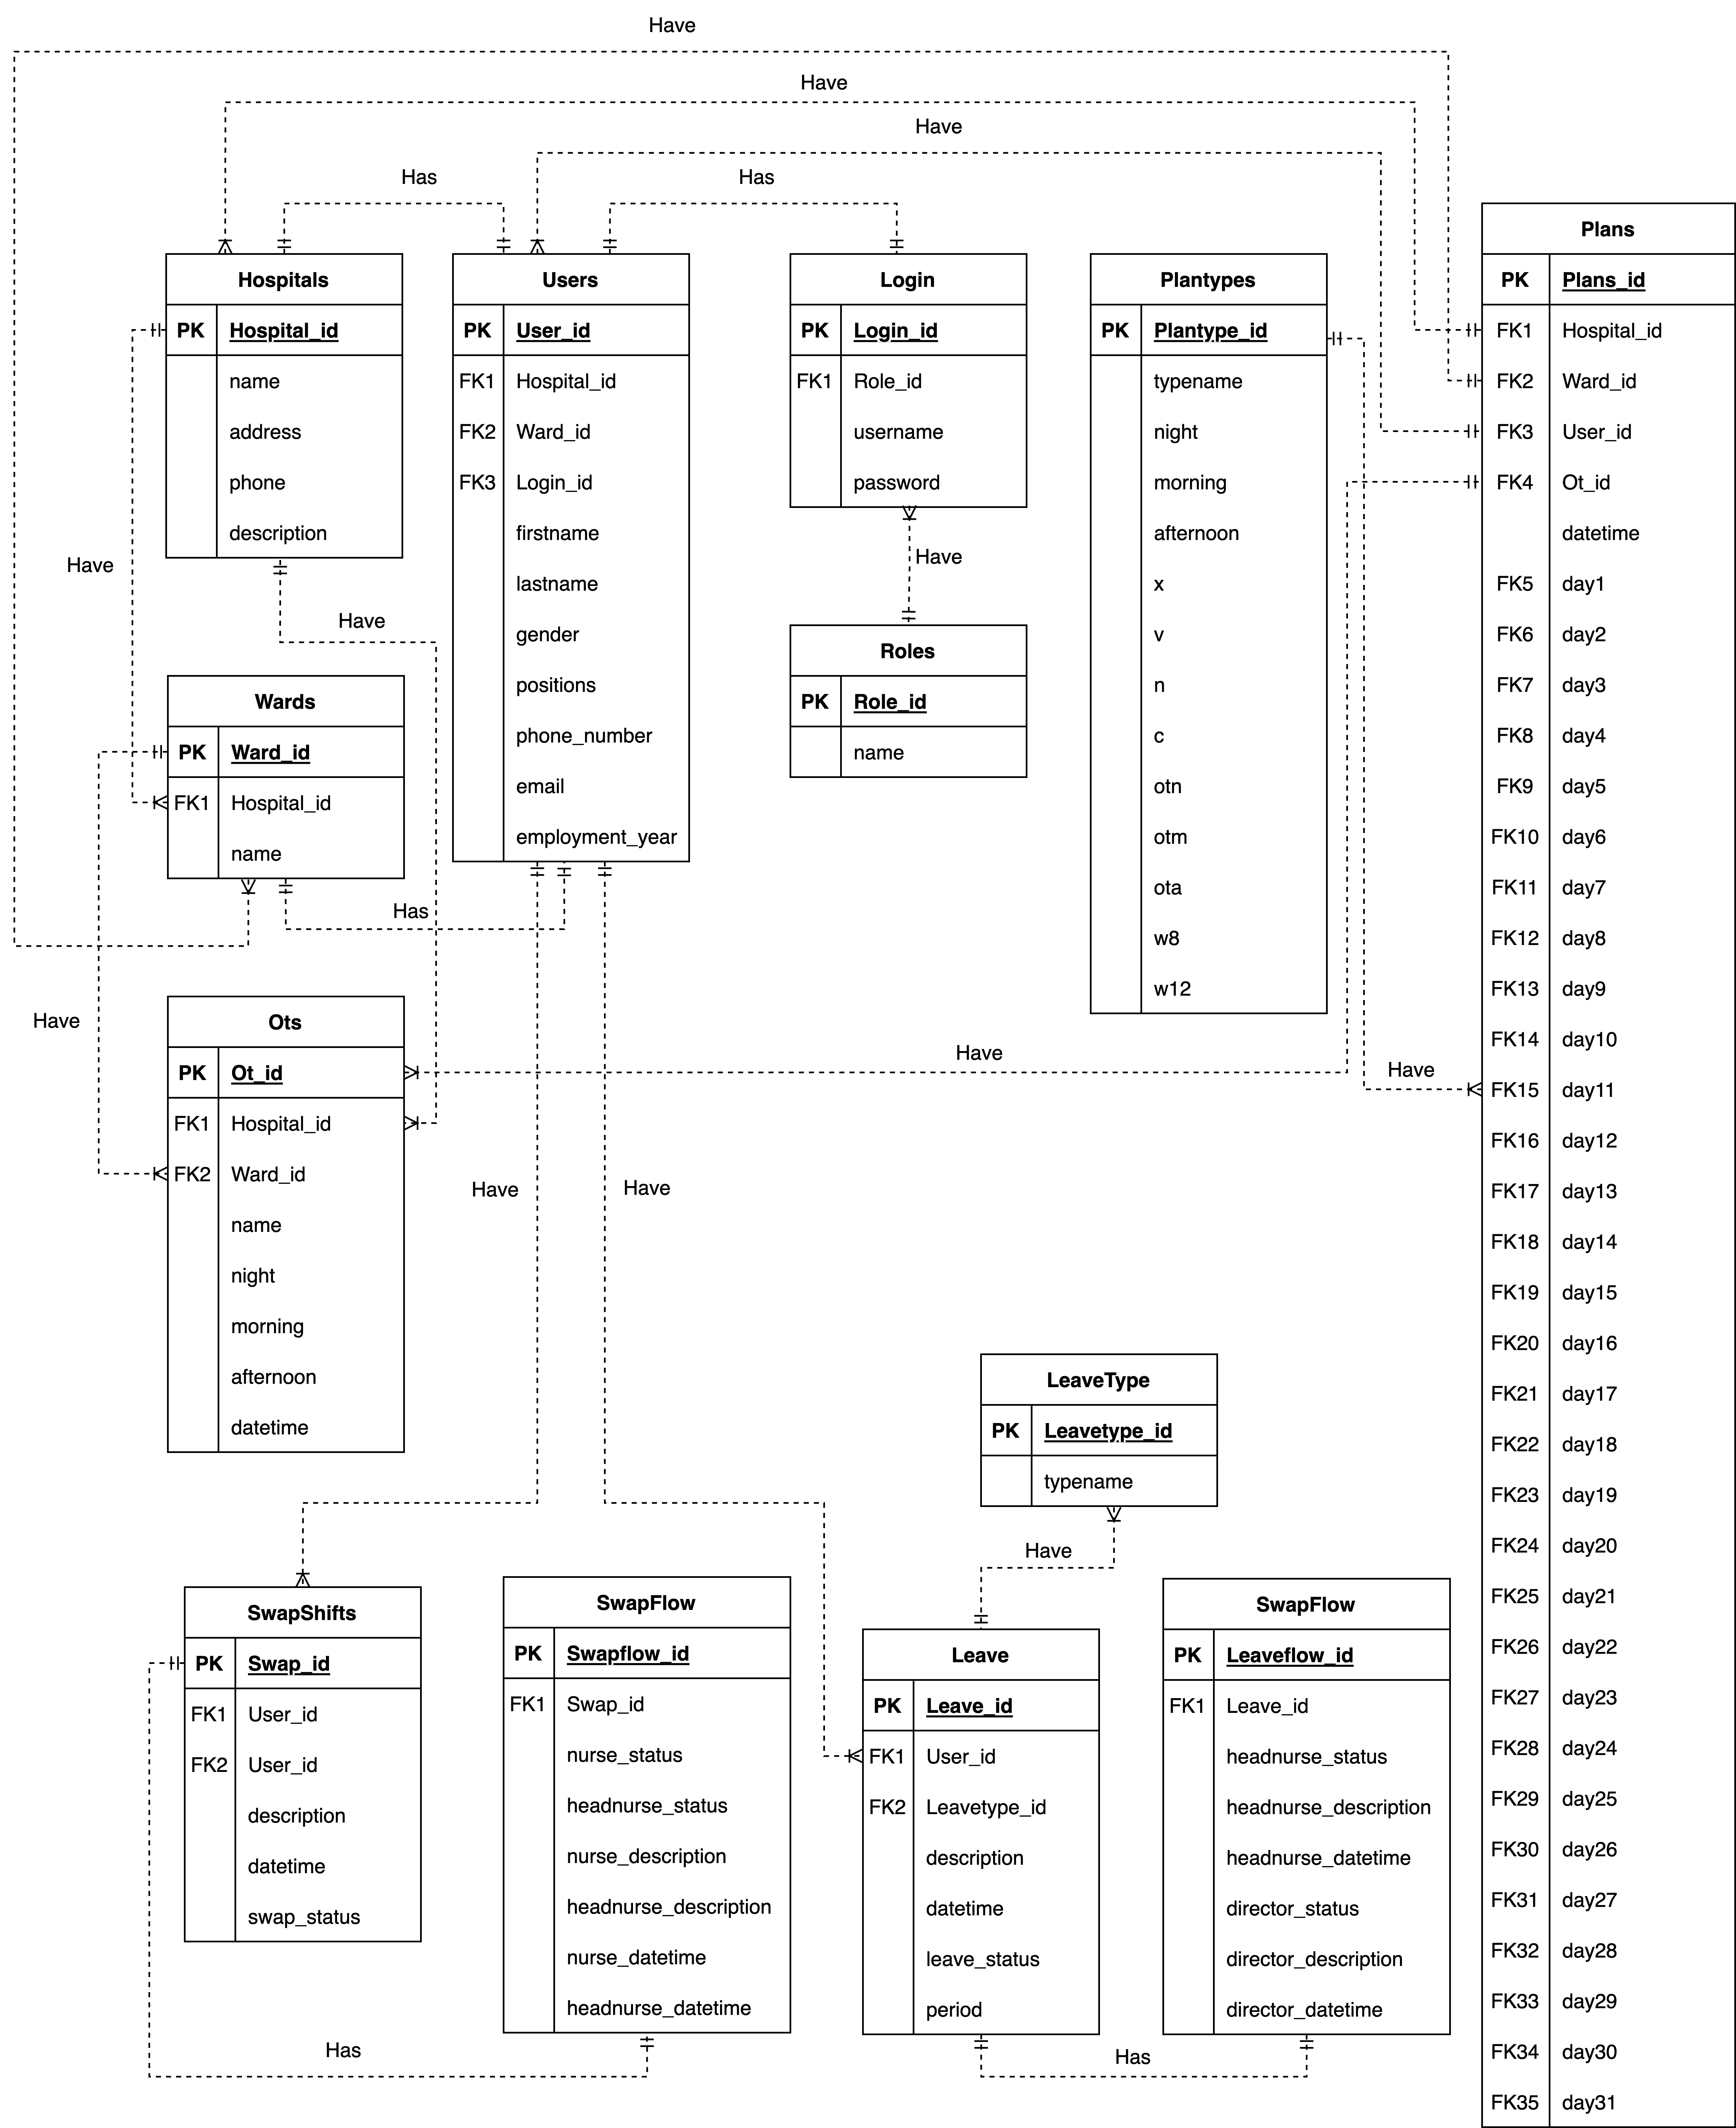
\includegraphics[width=1\textwidth]{ER.png}
   \caption{Entity-Relationship Diagram}
\end{figure}

\section{Entity-Relationship Description}

\section{การออกแบบหน้าจอแสดงผล}

\subsection{User 1}

\subsection{User 2}

\subsection{User 3}

\subsection{User 4}

\subsection{User 5}


\baselineskip=8mm
% \renewcommand{\thesubsection}{\thechapter.\arabic{subsection}}
\numberwithin{equation}{chapter}
\numberwithin{equation}{section}
\renewcommand{\thesubsection}{\arabic{subsection}.}
\renewcommand{\theequation}{\thesection.\arabic{equation}}
\renewcommand{\thesection}{}
\renewcommand{\thesubsubsection}{\thesubsection\arabic{subsubsection}.}

\begin{figure}[t]
    \centering
    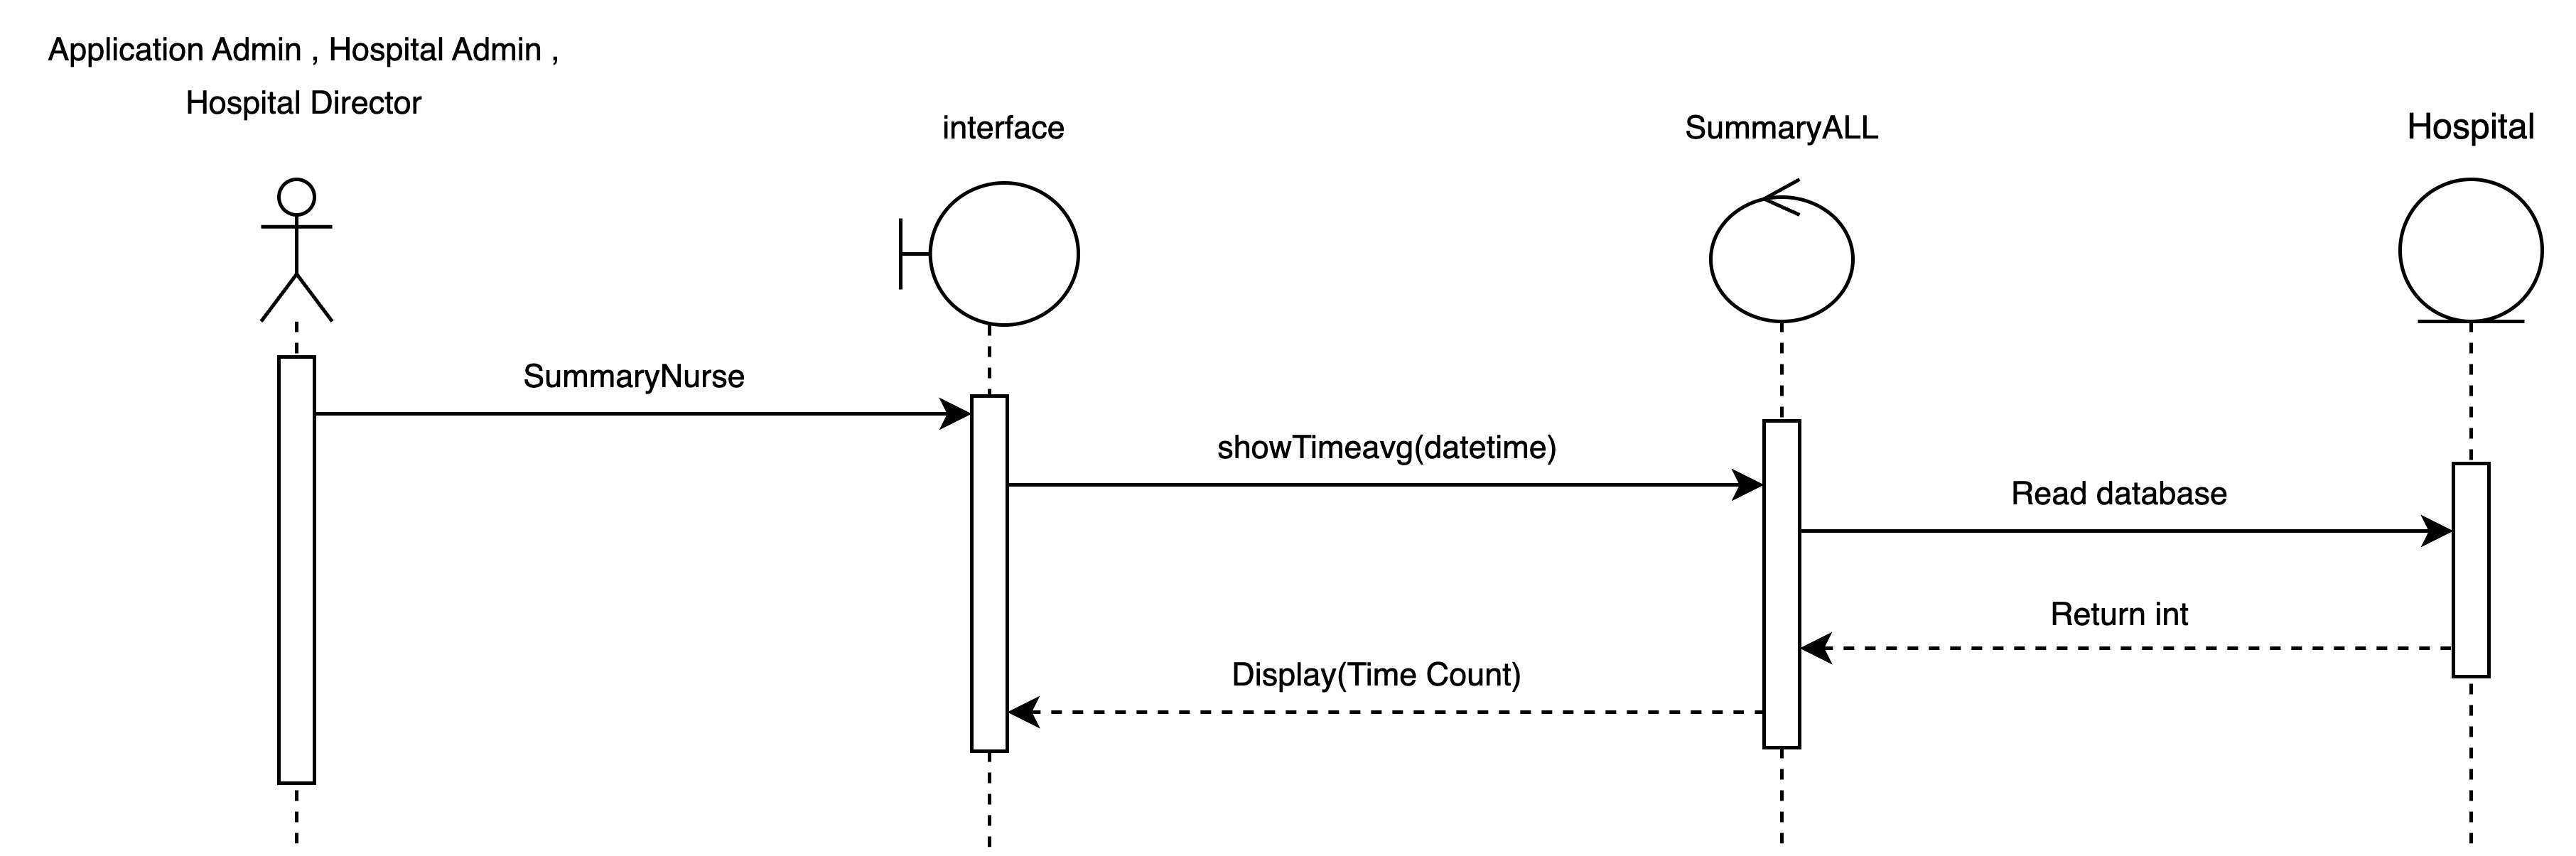
\includegraphics[width=0.8\textwidth]{Sequence 11.8.png}
    \caption{Use Case Diagram}
    \end{figure}
%\include{chap5}
%\include{chap6}
%\include{chap7}
%\include{chap8}
%\include{chap9}

\begin{thebibliography}{99}

\bibitem{wuhan:hupei}
    กรมควบคุมโรค. (2563). \textbf{คู่มือเจ้าหน้าที่สาธารณะสุขในการโต้ตอบภาวะฉุกเฉิน กรณีการระบาดโรคติดเชื้อไวรัสโคโรนา 2019 ในประเทศไทย.} ม.ป.ท.: ม.ป.พ.
\bibitem{nurse:covid}
    นราจันทร์ ปัญญาวุทโส, ปรัชญานันท์ เที่ยงจรรยา และประภาพร ชูกำเหนิด. (2565). \\วารสารมหาวิทยาลัยคริสเตียน. \textbf{ประสบการณ์ของพยาบาลวิชาชีพในการมีส่วนร่วม\\ด้านความปลอดภัยในภาวะวิกฤตของการแพร่ระบาดโรคโควิด 19 โรงพยาบาลหาดใหญ่ ประเทศไทย,} 28, 59-72.
\bibitem{nurse:Isolation}
    คณะกรรมาธิการการสาธารณะสุข วุฒิสภา. (2565). \textbf{ภาระงานและประสิทธิภาพของวิชาชีพพยาบาล ภายใต้สถานะการณ์การระบาดของโรค COVID 19.} ม.ป.ท.: ม.ป.พ.
\bibitem{people:nurse}
    สำนักงานปลัดกระทรวงสาธารณะสุข กระทรวงสาธารณะสุข. (2564). \textbf{สัดส่วนเจ้าหน้าที่ทางการแพทย์ต่อประชากร.} ม.ป.ท.: ม.ป.พ.
\bibitem{ngeaun:nurse}
    เกศินี กิตติบาล, อารี ชีวเกษมสุข และชูชาติ พ่วงสมจิตร์. (2564). วารสารพยาบาลโรคหัวใจและทรวงอก. \textbf{การจัดการความเหนื่อยล้าจากการทํางานของพยาบาลวิชาชีพ \\โรงพยาบาลพระนครศรีอยุธยา,} 32, 121-136.
\bibitem{tarang:nurse}
    กองการพยาบาล กระทรวงสาธารณะสุข. (2566). \textbf{แนวทางการบริหารการจัดตารางเวรหรือผลัด \\การเบิกเงินค่าตอบแทนนอกเวลาและค่าเวรหรือผลัดของพยาบาลวิชาชีพ พยาบาลเทคนิค ผู้ช่วยพยาบาล กระทรวงสาธารณสุข.} ม.ป.ท.: ม.ป.พ.
\bibitem{excel:headnurse}
    ปริวัฒณ์ อารีชาติ และคณะ. (2565). Thai Journal of Operations Research: TJOR. \textbf{ตัวแบบการจัดตารางเวรของเภสัชกรเพื่อลดความเหลื่อมล้ําของภาระงาน,} 10, 103-112
\end{thebibliography}



%\backmatter%%%%%%%%%%%%%%%%%%%%%%%%%%%%%%%%%%%%%%%%%%%%%%%%%%%%%%%

%\renewcommand{\bibname}{บรรณานุกรม}
%\bibliographystyle{myref}
%\nocite{*}
%\bibliography{References}


%%%%%%%%%%%%%%%%%%%%%%%%%%%%%%%%%%%%%%%%%
%%%%%%%%%%%%%%%%%%%%%%%%%%%%%%%%%%%%%%%%%
% CREATE THE BIBLIOGRAPHY  สร้างหน้าประวัติผู้เขียน
%%%%%%%%%%%%%%%%%%%%%%%%%%%%%%%%%%%%%%%%%
%%%%%%%%%%%%%%%%%%%%%%%%%%%%%%%%%%%%%%%%%
\clearpage

% not show ประวัติผู้วิจัย
% \renewcommand{\arraystretch}{1}
% \makebiography                          % Generate your biography page
% %\makeWorkExpr                           % Generate your work experiences
% \makeEduBG
%\makePublication
%\makePresentation

\end{document}

